\documentclass[11pt,a4paper]{article}

\usepackage[utf8]{inputenc}
\usepackage[T1]{fontenc}
\usepackage[french]{babel}
\usepackage[a4paper,margin=2.2cm]{geometry}
\usepackage{lmodern}
\usepackage{microtype}
\usepackage{graphicx}
\usepackage{float}
\usepackage{enumitem}
\usepackage{array}
\usepackage{longtable}
\usepackage{xcolor}
\usepackage{hyperref}

\hypersetup{
  colorlinks=true,
  linkcolor=black,
  urlcolor=blue,
  citecolor=black
}

\setlength{\parindent}{0pt}
\setlength{\parskip}{0.35em}
\setlength{\emergencystretch}{2em}
\setlength{\tabcolsep}{4pt}
\renewcommand{\arraystretch}{1.15}
\setlist[itemize]{leftmargin=1.2em,itemsep=0.12em,topsep=0.12em}

\newcommand{\code}[1]{\texttt{\detokenize{#1}}}
\newcommand{\figbox}[1]{%
  \fbox{\parbox{0.86\linewidth}{\centering\vspace{0.55cm}\textcolor{red!70!black}{#1}\vspace{0.55cm}}}%
}

\begin{document}
\sloppy
\pagenumbering{gobble}

\begin{titlepage}
\centering
\vspace*{2.0cm}

\includegraphics[width=0.33\linewidth]{img/Sciences_SU.png}\par
\vspace{2.0cm}
{\LARGE\bfseries TicketMet\par}
\vspace{0.2cm}
{\large Micro-projet Web\par}
\vspace{1.0cm}
{\large Jessy Fallavier\par}
\vspace{0.15cm}
{\large 21500607\par}
\vfill
{\large \today\par}
\end{titlepage}

\clearpage
\pagenumbering{roman}
\tableofcontents
\clearpage
\pagenumbering{arabic}

\section{Déploiement}

\begin{itemize}
  \item Le projet est conteneurisé avec Docker. C'est déployé sur mon VPS déjà en place, sans frais supplémentaires pour l'UE.
  \item Code source : \href{https://github.com/jessyfal04/ticketmet}{\code{github.com/jessyfal04/ticketmet}}.
  \item Site : \href{https://ticketmet.jessyfal04.dev}{\code{ticketmet.jessyfal04.dev}}.
  \item Les clés API sont lues depuis \code{.secrets/ticketmaster.mk}, chargé par le \code{Makefile}.
\end{itemize}

\section{Sujet de l'application}

TicketMet est une application web qui agrège les concerts en Europe et centralise leurs données importantes, comme la date, la salle, le plan et la setlist potentielle. L'idée est de garder un point d'entrée unique pour suivre les concerts, retrouver les informations utiles rapidement et éviter de jongler entre plusieurs sites.

L'application ajoute aussi une couche sociale. On peut suivre ses favoris avec une alerte de vente, recevoir des alertes de nouveauté, et utiliser les SNS (Social Network Service) pour faire du WTB (Want To Buy) / WTS (Want To Sell) ou simplement se retrouver avant un concert.

\section{Fonctionnalités}

\begin{itemize}
  \item Suivre des concerts, des artistes et des salles
  \item Consulter la liste des concerts en Europe
  \item Rechercher un concert par artiste ou salle
  \item Ouvrir la fiche d'un concert avec la date, la salle, la localisation, le plan si dispo et la setlist potentielle
  \item Utiliser Ticketmaster pour peupler la base de concerts
  \item Utiliser Setlist.fm pour enrichir une fiche quand la setlist est disponible
  \item Ajouter un concert en favoris pour activer l'alerte de vente
  \item Se mettre en WTB ou en WTS sur un concert
  \item Voir les autres personnes en WTB ou WTS pour un concert
  \item Activer une alerte de nouveaux concerts pour un artiste ou une salle
  \item Recevoir un mail de bienvenue à l'inscription
  \item Recevoir automatiquement des mails d'alertes
  \item Se connecter avec une passkey
  \item Renseigner ses SNS sur son profil
  \item Voir les SNS des gens qui vont au même concert
\end{itemize}






\section{Cas d'utilisation}

\begin{itemize}
  \item Scénario 1 : Alice met un concert en WTS, Bob se met en WTB ; ils reçoivent un mail de match, consultent la fiche du concert, récupèrent les SNS et se contactent pour l'échange de place.
  \item Scénario 2 : Eve active une alerte nouveauté sur NMIXX, reçoit un mail d'un nouveau concert, le met en favoris, puis reçoit l'alerte de vente quand les ventes ouvrent.
  \item Scénario 3 : Dave cherche un concert par salle, ouvre la fiche, consulte la setlist potentielle et ajoute le concert en favoris pour être alerté au lancement des ventes. Le jour des ventes il échoue à acheter une place, il se met en WTB.
  \item Scénario 4 : Lina consulte un concert depuis la recherche, elle copie le lien direct du concert puis l'envoie à son amie Lisa. Lisa ouvre la fiche avec le lien profond, consulte le plan de la salle et achète sa place.
  \item Scénario 5 : Sam se connecte avec une passkey, met à jour ses SNS dans son profil et retrouve ensuite les personnes qui vont au même concert.
\end{itemize}

\section{Schéma de base de données (\code{server/main/schema.sql})}

Le schéma sépare les concerts, les utilisateurs, les relations sociales, les alertes et l'état de synchronisation comme tel.

\begin{itemize}
  \item \textbf{\code{artists}} : \#\code{id} \code{INTEGER} / \code{name} \code{TEXT NN}
  \item \textbf{\code{venues}} : \#\code{id} \code{INTEGER} / \code{name} \code{TEXT NN} / \code{city} \code{TEXT NN} / \code{country} \code{TEXT NN}
  \item \textbf{\code{concerts}} : \#\code{id} \code{INTEGER} / \code{name} \code{TEXT NN} / \code{date} \code{TEXT NN} / \#\code{venue_id} \code{INTEGER NN ref(venues(id))} / \#\code{artist_id} \code{INTEGER NN ref(artists(id))} / \code{url} \code{TEXT NN} / \code{photo_url} \code{TEXT} / \code{seatmap_url} \code{TEXT} / \code{sale_start_datetime} \code{TEXT NN} / \code{created_at} \code{INTEGER}
  \item \textbf{\code{users}} : \#\code{id} \code{INTEGER} / \code{email} \code{TEXT NN UNIQUE} / \code{password_hash} \code{TEXT NN}
  \item \textbf{\code{sessions}} : \#\code{id} \code{INTEGER} / \#\code{user_id} \code{INTEGER NN ref(users(id))} / \code{token_hash} \code{TEXT NN UNIQUE} / \code{expires_at} \code{INTEGER NN}
  \item \textbf{\code{webauthn_credentials}} : \#\code{id} \code{INTEGER} / \#\code{user_id} \code{INTEGER NN ref(users(id))} / \code{credential_id} \code{TEXT NN UNIQUE} / \code{public_key} \code{TEXT NN} / \code{sign_count} \code{INTEGER} / \code{user_present} \code{BOOLEAN} / \code{user_verified} \code{BOOLEAN} / \code{backup_eligible} \code{BOOLEAN} / \code{backup_state} \code{BOOLEAN}
  \item \textbf{\code{webauthn_challenges}} : \#\code{id} \code{INTEGER} / \code{user_id} \code{INTEGER ref(users(id))} / \code{token_hash} \code{TEXT NN UNIQUE} / \code{kind} \code{TEXT NN CHECK (kind IN ('registration', 'login'))} / \code{session_data} \code{TEXT NN} / \code{expires_at} \code{INTEGER NN}
  \item \textbf{\code{user_sns}} : \#\code{user_id} \code{INTEGER NN ref(users(id))} / \#\code{sns} \code{TEXT NN}
  \item \textbf{\code{wt}} : \#\code{user_id} \code{INTEGER NN ref(users(id))} / \#\code{concert_id} \code{INTEGER NN ref(concerts(id))} / \code{type} \code{TEXT NN CHECK (type IN ('wtb', 'wts'))}
  \item \textbf{\code{favorites}} : \#\code{user_id} \code{INTEGER NN ref(users(id))} / \#\code{concert_id} \code{INTEGER NN ref(concerts(id))} / \code{created_at} \code{INTEGER}
  \item \textbf{\code{alerts}} : \#\code{id} \code{INTEGER} / \#\code{user_id} \code{INTEGER NN ref(users(id))} / \code{target_type} \code{TEXT NN CHECK (target_type IN ('artist', 'venue'))} / \code{target_id} \code{INTEGER NN} / \code{created_at} \code{INTEGER} / \code{UNIQUE(user_id, target_type, target_id)}
  \item \textbf{\code{notifications}} : \#\code{dedupe_key} \code{TEXT}
  \item \textbf{\code{setlists}} : \#\code{concert_id} \code{INTEGER NN ref(concerts(id))} / \#\code{song_order} \code{INTEGER NN} / \code{song_name} \code{TEXT NN}
  \item \textbf{\code{sync_ticketmaster}} : \#\code{id} \code{INTEGER CHECK (id = 1)} / \code{max_visibility} \code{TEXT NN}
\end{itemize}

\clearpage
\section{API Web}

J'utilise deux API externes, chacune avec un rôle précis : Ticketmaster pour peupler la base de concerts, puis Setlist.fm pour enrichir la fiche d'un concert quand la setlist est disponible.

\subsection{Ticketmaster}

\begin{itemize}
  \item Source des concerts, des images, des dates, des salles et des artistes.
  \item TicketMet interroge \code{events.json} par pays, filtre les nouveautés avec \code{publicVisibilityStartDateTime}, puis conserve les champs utiles pour construire la fiche concert.
  \begin{itemize}
    \item Champs utiles :
    \begin{itemize}
      \item Identifiant de l'event : \code{id}
      \item Nom de l'event : \code{name}
      \item Lien public : \code{url}
      \item Images : \code{images[].url}
      \item Date de concert : \code{dates.start.localDate / localTime / dateTime}
      \item Ouverture des ventes : \code{sales.public.startDateTime}
      \item Plan de salle : \code{seatmap.staticUrl}
      \item Salle : \code{_embedded.venues[0].id / name / city.name / country.countryCode}
      \item Artiste : \code{_embedded.attractions[0].id / name}
    \end{itemize}
  \end{itemize}
\end{itemize}

\subsection{Setlist.fm}

\begin{itemize}
  \item Source d'une setlist potentielle par artiste.
  \item TicketMet interroge \code{search/setlists}, prend la première setlist qui contient des songs, puis reconstruit la liste des titres à partir des chansons.
  \begin{itemize}
    \item Champs utiles :
    \begin{itemize}
      \item Liste de setlists \code{setlist[]}
      \item Noms des chansons d'une setlist \code{sets.set[].song[].name}
    \end{itemize}
  \end{itemize}
\end{itemize}

\clearpage
\section{Mise à jour}

Le rafraîchissement des données est découpé en jobs arrière-plan. Le serveur HTTP ne bloque pas sur ces traitements ; il sert les routes, pendant que les workers maintiennent la base et les notifications à jour.

\subsection{Sync Ticketmaster}

\begin{itemize}
  \item Le marqueur \code{publicVisibilityStartDateTime} sert de filtre de nouveauté, stocké dans \code{SyncTicketmaster.max_visibility}.
\item Les concerts sont récupérés puis insérés par pays, avec les pays frontaliers à la France : \code{DE}, \code{FR}, \code{BE}, \code{NL}, \code{LU}, \code{CH}, \code{AD}, \code{GB}, \code{IT}, \code{MC} et \code{ES}. Les données françaises sont limitées car \textbf{Ticketmaster France} est en réalité \textbf{Ticketnet}, dont le site est différent.
  \item Le job tourne en goroutine, démarre tout de suite, puis se relance toutes les 15 minutes avec la clé Ticketmaster fournie par le shell \code{TICKETMASTER_API_KEY}.
\item Un nettoyage est effectué : on garde les events avec un nom d'event, une salle ou un artiste exploitable, une seule photo avec bonus 16:9 si possible, et on ignore les dates de vente aberrantes avant 2000.
\end{itemize}

\subsection{Radar d'alertes}

\begin{itemize}
  \item Le radar vérifie les alertes de nouveauté, les alertes de vente et les matches WTB/WTS.
  \item Les notifications déjà envoyées sont dédupliquées via \code{notifications.dedupe_key}.
  \item Quand un événement déclenche une alerte, le worker prépare le mail correspondant sans bloquer les handlers HTTP.
\end{itemize}

\subsection{Setlist}

\begin{itemize}
  \item La setlist est d'abord lue dans le cache SQLite.
  \item Si elle manque et que \code{SETLISTFM_API_KEY} est fourni, le serveur interroge Setlist.fm puis complète la réponse.
\end{itemize}

\section{Requêtes implémentées}

\subsection{Routes de consultation}

\small
\begin{table}[H]
\centering
\caption{Routes de consultation}\label{tab:routes_consultation}
\begin{tabular}{|>{\raggedright\arraybackslash}m{0.28\linewidth}|>{\raggedright\arraybackslash}m{0.48\linewidth}|>{\raggedright\arraybackslash}m{0.18\linewidth}|}
\hline
\textbf{REQUÊTES} & \textbf{DESCRIPTION} & \textbf{RÉPONSE} \\
\hline
GET /healthz & healthcheck serveur & texte brut ok, code 200 \\
\hline
GET /api/concerts avec artistID, venueID, country, status et page & liste des concerts, avec filtre optionnel par artiste, salle, pays et pagination & liste de DisplayConcert \\
\hline
GET /api/concerts par identifiant & détail d'un concert & DisplayConcert \\
\hline
GET /api/artists & liste des artistes & liste d'Artist \\
\hline
GET /api/venues & liste des salles & liste de Venue \\
\hline
GET /api/favorites par concert & voir les SNS des gens qui vont au même concert & SNS des personnes du même concert \\
\hline
GET /api/setlist par concert & voir la setlist potentielle d'un concert & liste de chansons potentielles \\
\hline
GET /api/wt par concert & voir les WTB et WTS liés à un concert & WTB, WTS et compteurs \\
\hline
\end{tabular}
\end{table}
\normalsize

\subsection{Routes d'authentification}

\small
\begin{table}[H]
\centering
\caption{Routes d'authentification}\label{tab:routes_auth}
\begin{tabular}{|>{\raggedright\arraybackslash}m{0.28\linewidth}|>{\raggedright\arraybackslash}m{0.48\linewidth}|>{\raggedright\arraybackslash}m{0.18\linewidth}|}
\hline
\textbf{REQUÊTES} & \textbf{DESCRIPTION} & \textbf{RÉPONSE} \\
\hline
POST /api/auth/register & créer un compte email/password et ouvrir une session cookie & utilisateur connecté \\
\hline
POST /api/auth/login & se connecter avec email/password & utilisateur connecté \\
\hline
POST /api/auth/logout & révoquer la session courante & statut 204 \\
\hline
DELETE /api/auth/unregister & supprimer son compte avec confirmation password & statut 204 \\
\hline
GET /api/auth/me & récupérer l'utilisateur connecté & utilisateur connecté \\
\hline
GET /api/auth/email-exists avec email & vérifier si un email existe & oui ou non \\
\hline
POST /api/auth/passkeys/ register/begin & commencer l'ajout d'une passkey pour l'utilisateur connecté & options WebAuthn \\
\hline
POST /api/auth/passkeys/ register/finish & valider et stocker la passkey créée & confirmation OK \\
\hline
POST /api/auth/passkeys/ login/begin & commencer une connexion passkey sans email & options WebAuthn \\
\hline
POST /api/auth/passkeys/ login/finish & valider la passkey et ouvrir une session cookie & utilisateur connecté \\
\hline
GET /api/auth/passkeys & lister les passkeys de l'utilisateur connecté & liste de passkeys \\
\hline
DELETE /api/auth/passkeys par credentialId & supprimer une passkey de l'utilisateur connecté & statut 204 \\
\hline
\end{tabular}
\end{table}
\normalsize

\subsection{Routes d'interaction et profil}

\small
\begin{table}[H]
\centering
\caption{Routes d'interaction et profil}\label{tab:routes_interaction}
\begin{tabular}{|>{\raggedright\arraybackslash}m{0.28\linewidth}|>{\raggedright\arraybackslash}m{0.48\linewidth}|>{\raggedright\arraybackslash}m{0.18\linewidth}|}
\hline
\textbf{REQUÊTES} & \textbf{DESCRIPTION} & \textbf{RÉPONSE} \\
\hline
POST ou DELETE /api/favorites par concert & ajouter ou retirer un favori ; cela active ou désactive l'alerte de vente & statut 204 \\
\hline
POST ou DELETE /api/wt par concert avec type wtb ou wts & se mettre ou retirer en WTB ou WTS ; POST remplace l'autre statut du même user sur le même concert, et un concert expiré renvoie 409 & statut 204 \\
\hline
POST /api/alerts avec targetType et targetId & créer une alerte de nouveauté & confirmation OK \\
\hline
DELETE /api/alerts par alertId & retirer une alerte & statut 204 \\
\hline
GET /api/me & voir le profil complet & profil complet \\
\hline
PATCH /api/me & modifier le profil, ici les SNS & profil mis à jour \\
\hline
\end{tabular}
\end{table}
\normalsize

\subsection{Sortie JSON}

\begin{itemize}
  \item Requête :
\begin{verbatim}
GET /api/auth/passkeys
\end{verbatim}
  \item Struct :
\begin{verbatim}
type passkeyListResponse struct {
    Passkeys []model.PublicPasskey
}
\end{verbatim}
  \item Réponse JSON :
\begin{verbatim}
{
  "Passkeys": [
    {
      "CredentialID": "c29tZS1jcmVkZW50aWFsLWlk",
      "SignCount": 12
    }
  ]
}
\end{verbatim}
  \item Explication :
  \begin{itemize}
    \item \code{passkeyListResponse} est la struct racine envoyée par \code{writeJSON}.
    \item \code{Passkeys} est une liste de \code{model.PublicPasskey}.
    \item Chaque passkey publique garde seulement \code{CredentialID} et \code{SignCount}.
  \end{itemize}
\end{itemize}

\section{Description serveur}

Le serveur Go s'appuie sur \code{net/http} pour l'HTTP et sur \code{database/sql} pour SQLite. J'ai gardé les routes proches des données, et les requêtes SQL restent visibles dans les handlers et dans les jobs.

Le démarrage se fait dans \code{server/main/main.go}. Ce fichier ouvre la base, prépare les canaux et lance les workers en arrière-plan avant de servir HTTP. La façade des routes reste dans \code{server/api/api.go}, qui assemble les handlers au même endroit.

La base SQLite persiste dans \code{/app/data/ticketmet.sqlite3} en production.

Les scanners partagés vivent dans \code{server/model/scan.go} avec les structs dans \code{server/model/models.go} ; ça permet garder les requêtes SQL simples et proches des données.

\subsection{Architecture du serveur}

\begin{verbatim}
server
|-- api
|   |-- alerts.go
|   |-- api.go
|   |-- artists.go
|   |-- auth.go
|   |-- concerts.go
|   |-- favorites.go
|   |-- healthz.go
|   |-- passkeys.go
|   |-- profile.go
|   |-- setlist.go
|   |-- venues.go
|   |-- wt.go
|-- job
|   |-- alertradar.go
|   |-- database.go
|   |-- mailserver.go
|   |-- setlistfm.go
|   |-- ticketmaster.go
|   |-- worker.go
|-- main
|   |-- main.go
|   |-- schema.sql
|-- model
    |-- models.go
    |-- scan.go
\end{verbatim}

\subsection{Tableau des jobs}

\small
\begin{table}[H]
\centering
\caption{Tableau des jobs}\label{tab:jobs}
\begin{tabular}{|>{\raggedright\arraybackslash}m{0.24\linewidth}|>{\raggedright\arraybackslash}m{0.18\linewidth}|>{\raggedright\arraybackslash}m{0.30\linewidth}|>{\raggedright\arraybackslash}m{0.18\linewidth}|}
\hline
\textbf{Fichier} & \textbf{Déclenchement} & \textbf{Rôle} & \textbf{Flux} \\
\hline
server/job/database.go & en continu & exécute les requêtes SQL en série & dbChan \\
\hline
server/job/ticketmaster.go & au démarrage puis toutes les 15 min & synchronise les concerts Ticketmaster & HTTP GET + dbChan \\
\hline
server/job/setlistfm.go & à la demande via /api/setlist/{id} & lit le cache puis interroge Setlist.fm si besoin & setlistChan + dbChan + HTTP GET \\
\hline
server/job/alertradar.go & au démarrage puis toutes les 1 min & détecte les alertes, les ventes et les matches WTB/WTS & dbChan + mailChan \\
\hline
server/job/mailserver.go & en continu & consomme les mails en file buffered et les envoie en SMTP & mailChan + SMTP \\
\hline
\end{tabular}
\end{table}
\normalsize

\clearpage
\subsection{Mail applicatif}

Le mailserver envoie le mail de bienvenue à l'inscription, puis les mails d'alertes du radar.

\begin{figure}[H]
\centering
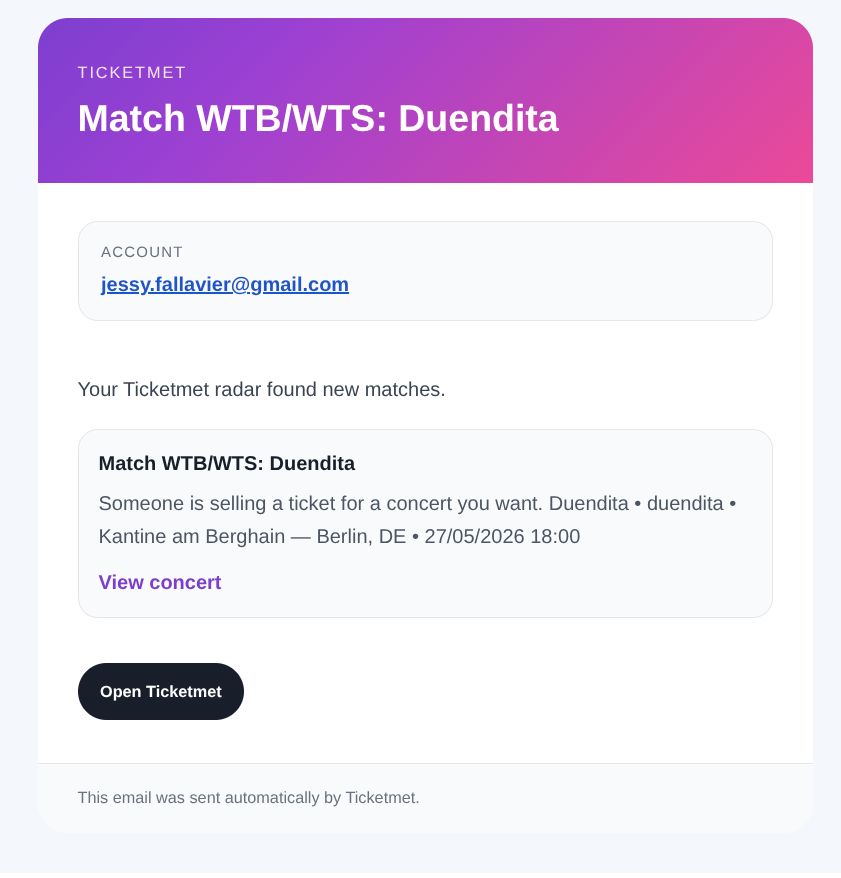
\includegraphics[width=0.78\linewidth]{img/mail.png}
\caption{Mail de bienvenue et mail d'alertes}
\end{figure}

\clearpage
\section{Description client}

Le client est une monopage en JavaScript : \code{jQuery} gère les appels AJAX, les événements DOM et le scroll ; \code{Bulma CSS} porte la structure visuelle (les forms, les buttons, les tags et les blocs de notifications) ; \code{React} / \code{ReactDOM} restent limités à quelques islands ciblées. Le code est découpé entre \code{client/lib/script.js} pour l'état partagé et les helpers, puis \code{client/lib/account.js}, \code{client/lib/search.js}, \code{client/lib/detail.js}, \code{client/lib/passkeys.js} pour les écrans spécifiques.

\subsection{Architecture du client}

\begin{verbatim}
client
|-- img
|   |-- concert.png
|-- index.html
|-- lib
|   |-- account.js
|   |-- detail.js
|   |-- passkeys.js
|   |-- script.js
|   |-- search.js
|-- style
    |-- bulma.min.css
    |-- style.css
\end{verbatim}

\clearpage
\subsection{Plan du site par écran}

\subsubsection{searchView}

Le point d'entrée de l'application affiche les concerts, les filtres et la pagination. Au chargement, l'app vérifie l'état du serveur, la session et la disponibilité des listes de base, puis elle lance la première recherche.

\begin{itemize}
  \item Les filtres artiste, salle, pays et période relancent la recherche.
  \item Le scroll déclenche le chargement de la page suivante.
  \item Le bouton \code{Clear} remet l'état à zéro.
  \item Le bouton \code{Open} d'une carte ouvre la fiche concert.
  \item AJAX : \code{GET /healthz}, \code{GET /api/auth/me}, \code{GET /api/artists}, \code{GET /api/venues}, \code{GET /api/concerts?artistID=...&venueID=...&country=all|<code>&status=future|all&page=...}
  \item AJAX : \code{POST /api/alerts?targetType=artist|venue&targetId=...} pour créer une alerte depuis la recherche
\end{itemize}

\begin{figure}[H]
\centering
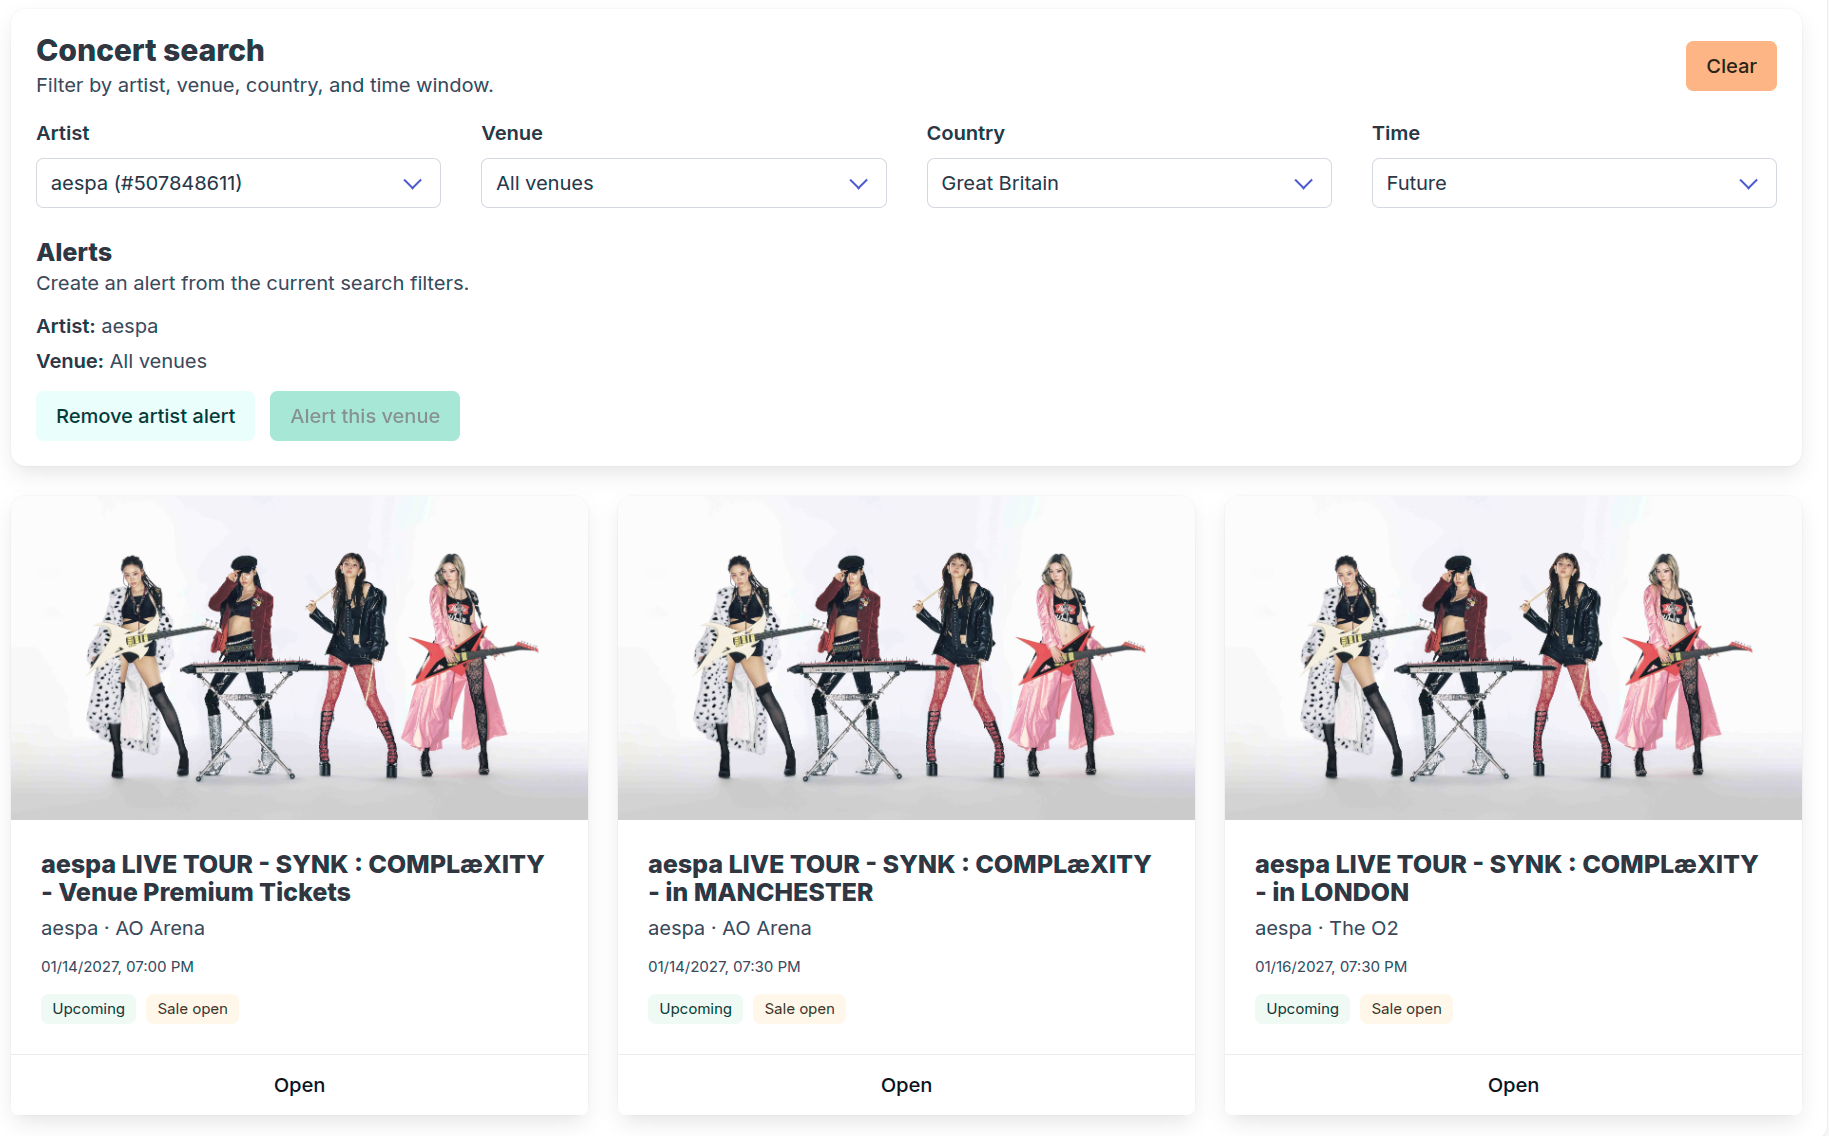
\includegraphics[width=0.96\linewidth]{img/search_aespa_uk.png}
\caption{Vue searchView}
\end{figure}

\clearpage
\subsubsection{detailView}

La fiche concert s'ouvre depuis la recherche ou via le lien profond \code{?concert=...}. Elle rassemble le détail du concert, la setlist potentielle, les SNS, les favoris et les actions WTB/WTS.

\begin{itemize}
  \item \code{renderConcert()} remplit la fiche principale.
  \item \code{loadConcertFeatures()} lance les compléments autour de la setlist, des SNS et des statuts WTB/WTS.
  \item Les boutons \code{Share}, favoris, WTB et WTS déclenchent les callbacks associés.
  \item AJAX : \code{GET /api/concerts/{id}}, \code{GET /api/setlist/{id}}, \code{GET /api/favorites/{id}}, \code{GET /api/wt/{id}}
  \item AJAX : \code{POST/DELETE /api/favorites/{id}}, \code{POST/DELETE /api/wt/{id}?type=wtb|wts}
  \item AJAX : \code{GET /api/me} après une mise à jour de profil ou d'action si l'utilisateur est connecté
\end{itemize}

\begin{figure}[H]
\centering
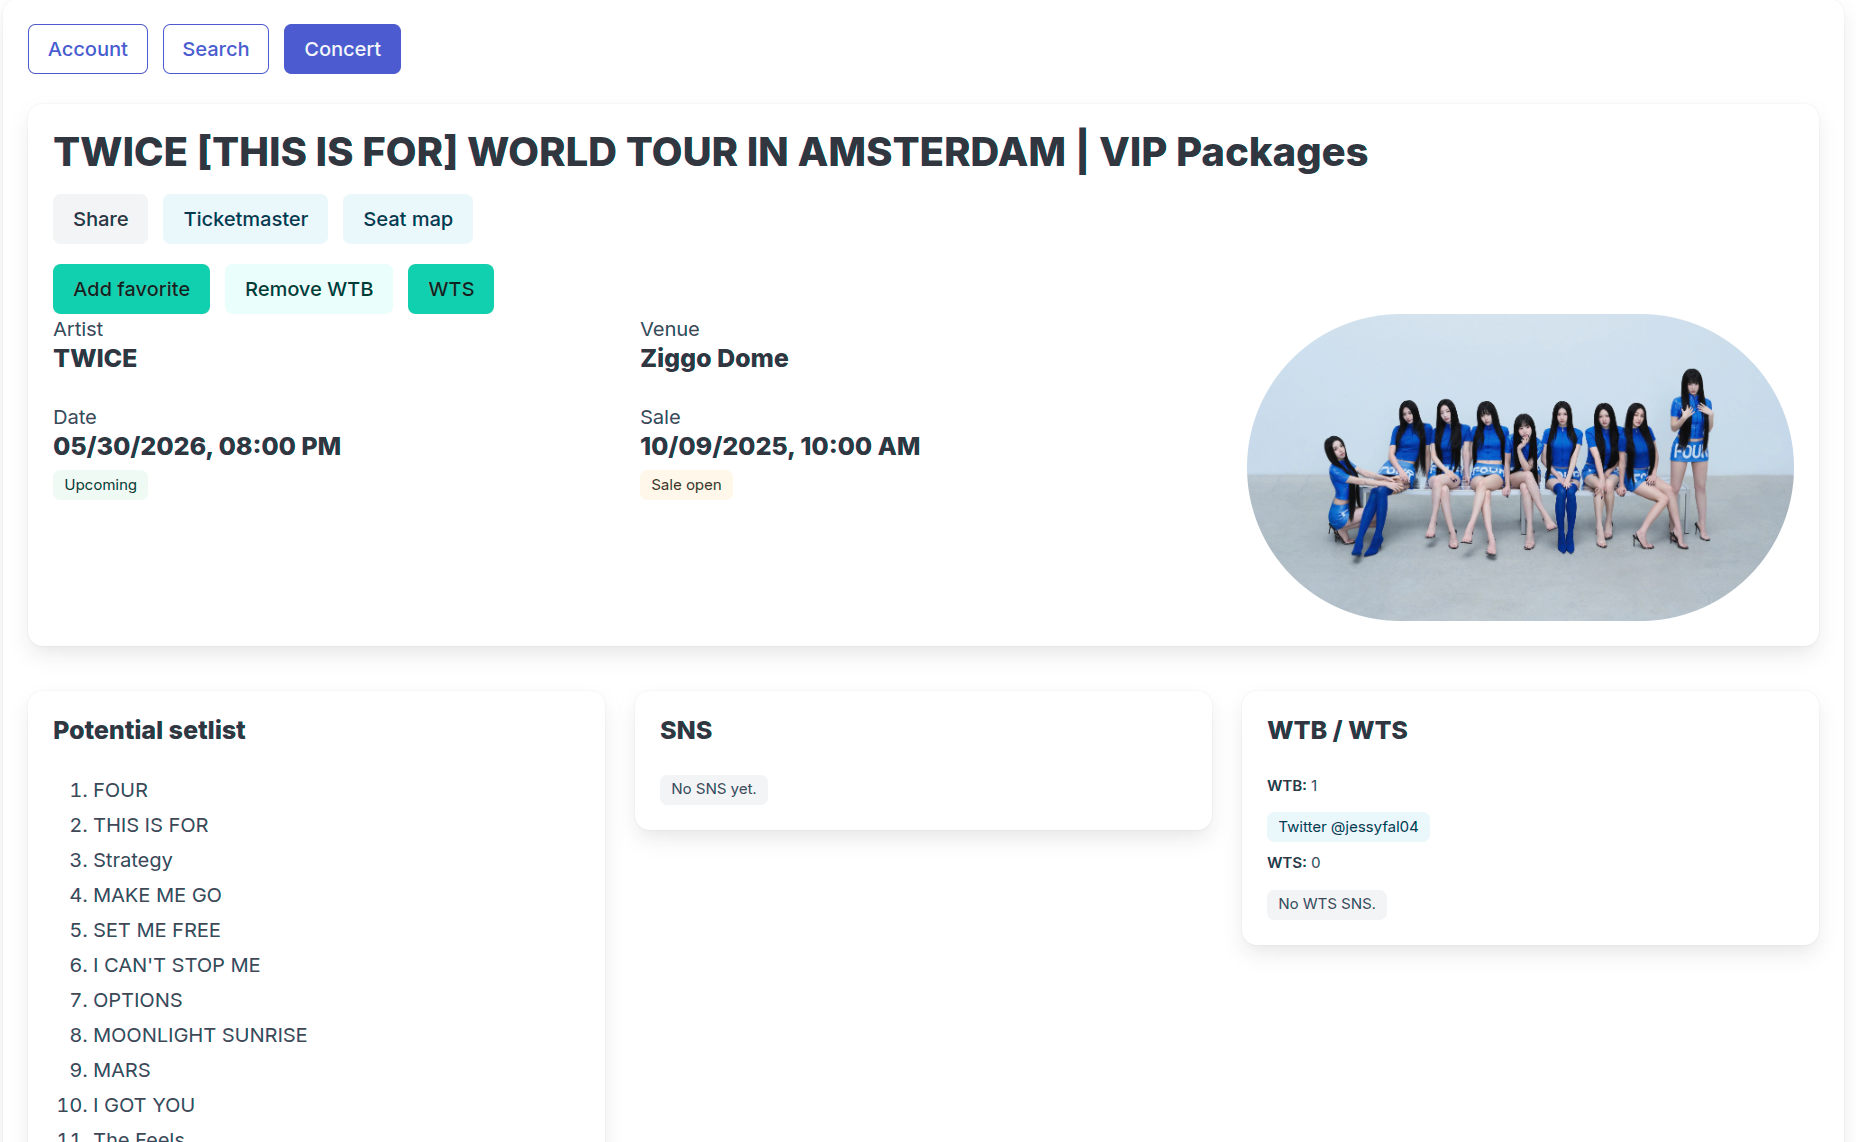
\includegraphics[width=0.96\linewidth]{img/details_twice.png}
\caption{Vue detailView}
\end{figure}

\clearpage
\subsubsection{accountView}

L'écran compte affiche soit le bloc sign in / register / passkey login, soit le profil utilisateur avec ses passkeys, ses favoris, ses WT et ses alertes.

\begin{itemize}
  \item Quand l'utilisateur est déconnecté, il voit les formulaires d'inscription, de connexion et de connexion passkey.
  \item Quand l'utilisateur est connecté, il voit son profil, ses passkeys, ses favoris, ses WT, ses alertes et la zone de suppression du compte.
  \item \code{showView("accountView")} recharge les données utiles avant d'afficher la vue.
  \item AJAX : \code{POST /api/auth/register}, \code{POST /api/auth/login}, \code{POST /api/auth/logout}, \code{DELETE /api/auth/unregister}
  \item AJAX : \code{GET /api/auth/email-exists}, \code{GET /api/auth/me}, \code{GET /api/me}, \code{PATCH /api/me}
  \item AJAX : \code{GET /api/auth/passkeys}, \code{POST /api/auth/passkeys/register/begin}, \code{POST /api/auth/passkeys/register/finish}, \code{POST /api/auth/passkeys/login/begin}, \code{POST /api/auth/passkeys/login/finish}, \code{DELETE /api/auth/passkeys/{credentialId}}
  \item AJAX : \code{DELETE /api/alerts/{alertId}}
\end{itemize}

\begin{figure}[H]
\centering
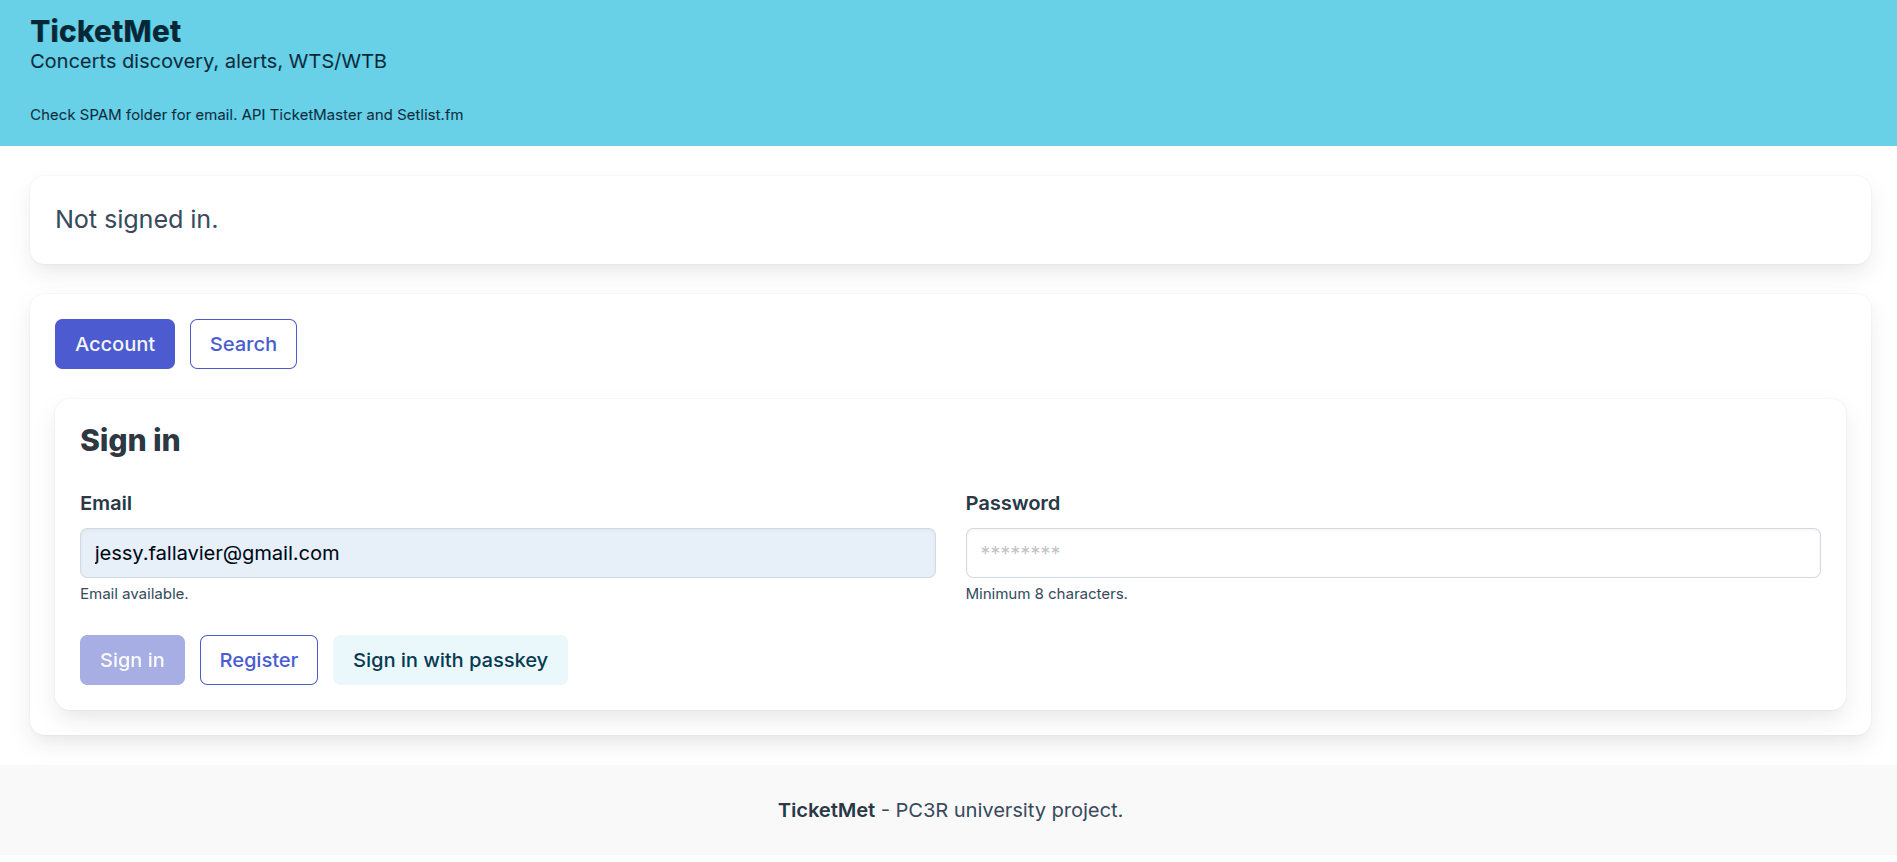
\includegraphics[width=0.96\linewidth]{img/account_register.png}\par\medskip
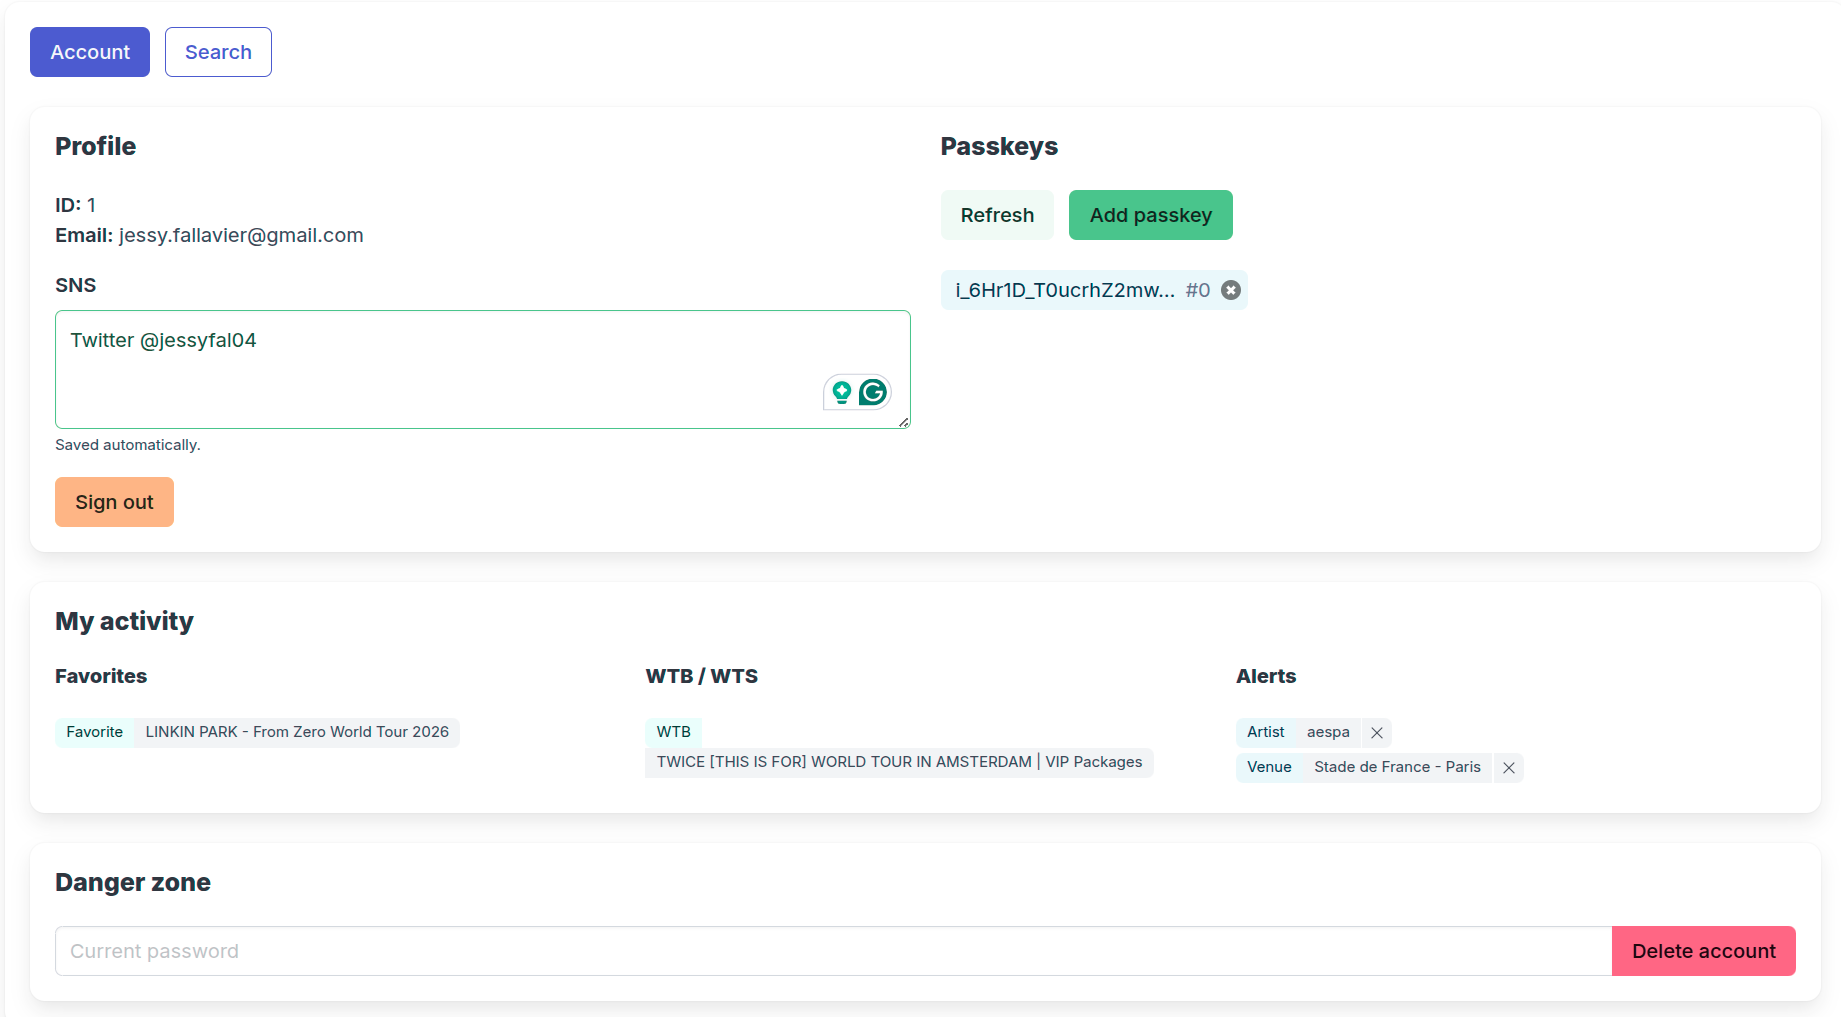
\includegraphics[width=0.96\linewidth]{img/account_logged.png}
\caption{Vue accountView non connecté (en haut) et connecté (en bas)}
\end{figure}

\section{Schéma global du système}

Le schéma ci-dessous résume la chaîne principale : client, AJAX, serveur, jobs, bases et APIs externes.

\begin{figure}[H]
\centering
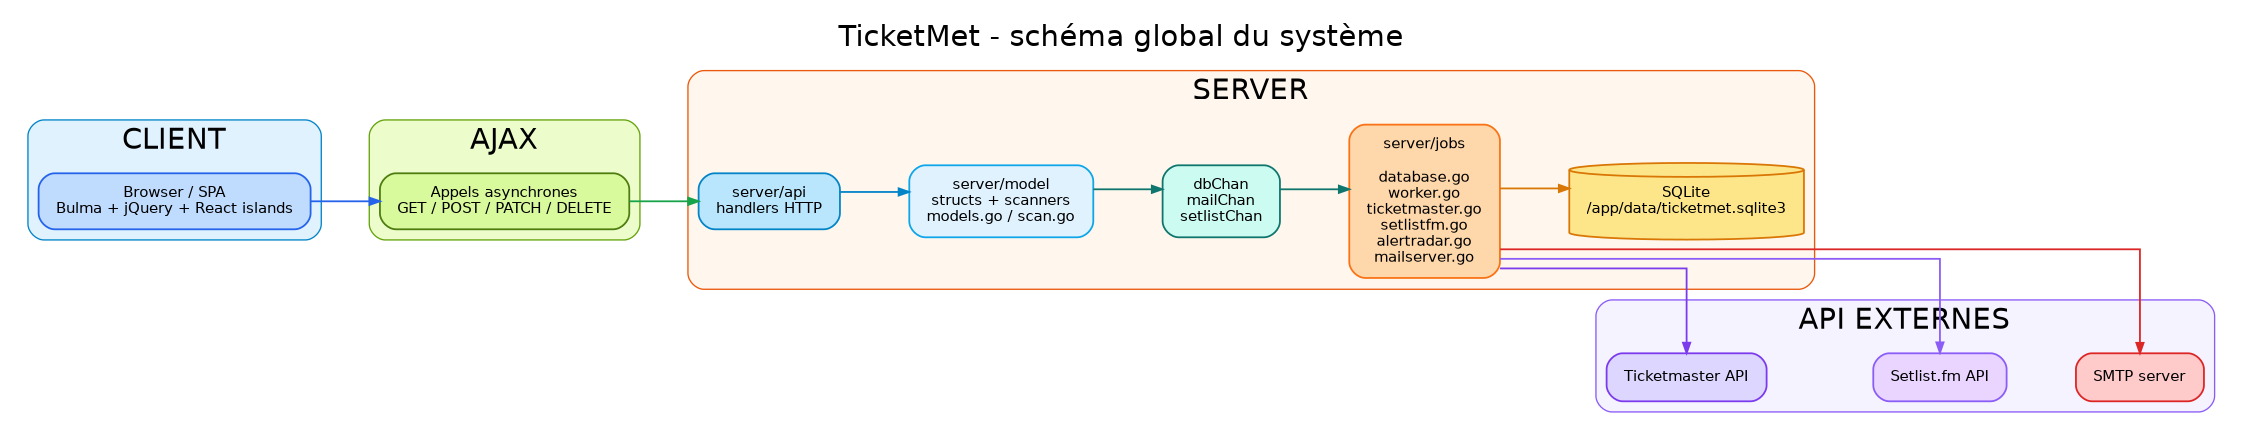
\includegraphics[width=\linewidth]{img/schema_global.png}
\caption{Schéma global du système}
\label{fig:schema-global}
\end{figure}

\section{Sécurité}

\begin{itemize}
  \item Les mots de passe sont hashés avec \code{bcrypt} avant stockage.
  \item Les sessions sont stockées en base sous forme de hash \code{token_hash}.
  \item Les challenges WebAuthn sont aussi stockés sous forme de hash avec une durée de vie courte.
  \item La passkey est utilisée pour la connexion sans mot de passe.
  \item Le cookie de session est \code{HttpOnly} et passe en \code{Secure} quand la requête est en HTTPS.
  \item L'email est validé à l'inscription.
  \item Le mot de passe doit faire au moins 8 caractères.
  \item L'expiration de session est vérifiée côté serveur avant de considérer comme l'utilisateur connecté.
\end{itemize}

\section{Perspectives futures}

\begin{itemize}
  \item Notification push via Firebase
  \item Job additionnel pour retirer les sessions et les challenges passkey expirés
  \item Passage plus large en React ou en TypeScript, surtout sur la vue de détail d'un concert qui reste le plus gros bloc
  \item Mise en place d'une Progressive Web App
\end{itemize}

\clearpage
\section{Références et IA}

Mes dépôts GitHub d'anciens projets \href{https://github.com/jessyfal04/avotey}{\code{avotey}} pour la partie visuelle et \href{https://github.com/jessyfal04/webauthnnotes}{\code{webauthnnotes}} pour la partie Passkey.
\subsection*{Utilisation de l'IA}

Dans une démarche de transparence, voici les prompts que j'ai demandé à ChatGPT.

\begin{verbatim}
- Explique moi comment je peux faire ce serveur en Go, la nomenclature de l'appli, comme on va garder les infos de manière persistante, en utilisant json et net/http, comment on va coder les requetes, comment on va pouvoir tester avec des codes bash telnet, dans un premier temps avec des dummy base, des classes pour stocker les données ?
- Selon notes.md, donne des struct go qui représente ces données / id en int /
- Give a dummyData function for the app with several venues...
- Donne 2 template pour les requetes artists et venues; Donne 2 template de test.sh pour artists et venues + avec Accor et NMIX
- Donne la nomclature d'une fonction qui prends un string optionnel et renvoi nil ou le int
- A quoi ressemble un sync pour l'API ticketmaster dans app.md ?
- Lis le frontend que j'ai fais pour une appli de vote (docs/avotey) et applique le pour l'appli ticketmet (client) - suis bien toutes les spécifications de app.md
- Clone https://github.com/jgthms/bulma/tree/741da22368cd548111224983a1c3ece8954fe8cc/docs de la doc de bulma et vérif quelles règles css on peut retirer.
- Quel spécification pour appli web ? genre je veux que tt sois à jour et bien faire genre bulma et les autres dépendances go, comment on fait ?
- Quels étapes pour déployer sur mon VPS avec Docker ? En mode auto dès que ya une modif.
- Comment ajouter du react ici, quels cas d'usage?
- Une base de données sqlite3 c bon ici nan?
- Modifie model pour que ça prenne de la db, et donne moi les requêtes sql type
- dans artist et concert et venues ya du code qui se répète nan, dans la structure. Comment factoriser tt ça ? Genre c'est vraiment la même dynamique à chaque fois, fait en sorte de paramétriser tt ça en un gros helpeur nan ?
- Il ya un mélange de nom anglais et de nom français, je ne veux garder que l'anglais.
- Automatise le resync Ticketmaster tt les 15 minutes, ça doit utiliser le schema sql et le readme
- Using my 2 old projects docs/src avotey (php) and webauthnnotes (python), adapt into go, you have the routes in api.go and README.md; same behavior!
- Same for the frontend I want to keep the same logic as docs/src avotey (php) and webauthnnotes (python) ! js file and html
- Passkey inconsistency I need to store flags?
- Read the readme file, add placeholder for the remaining functions
- I prefer to have response struct instead of map, modify.
- How can I have a job with a timer via a chan?
- Imagine a beautiful html email template with a dedicated place for the mail
- Crée httpGetIntParam sous le même format que httpGetStringParam
- Do ssh vps, I have a pb the docker-deploy, it keeps restarting.
- I'll have a job folder with all the workers. You think I can mutualize some code?
- How could I create a frontend monopage Bulma inspired by avotey+webauthnnotes, I want all my backend features.
- Which scanner can be created / deleted. Maybe bool and string ?
- I really need to create a date field for the favorites alerts in order to avoid sending one immediately if sales are already open?
- Regarde chaque requête SQL et vérif si elle peut etre simpliée en gardant le même comportement. Je ne veux AUCUNE erreur. Tout en restant compact!
- Voici mes codes javascript. Donne moi une idée de mini bouts qu'on peut mettre en mode React. Fais une liste des bons candidats et donne moi leur mini code.
- Here's my files, please comment each function for exemple
\end{verbatim}

\end{document}
